\documentclass[10pt,spanish,a4paper,openany,notitlepage]{article}
%-------------------------------------Paquetes-----------------------------------------------------------------------
\usepackage[spanish,es-tabla]{babel}  % Traduce los textos a castellano
\usepackage[utf8]{inputenc}	% Permite escribir directamente áéíóúñ
\usepackage{t1enc}      	% Agrega caracteres extendidos al font
\usepackage{amsmath} 	%Permite imprimir mas opcciones matematicas
\usepackage{graphicx}	%Permite agregar imagenes al informe
\usepackage{multicol}  %Permite dividir el texto en varias columnas
\usepackage{float} 	%Permite utilizar H para colocar las imagenes en un lugar especifico 
\usepackage{units}
\usepackage{circuitikz}
\usepackage{caption}
\usepackage{subcaption}
\usepackage{sidecap}
\usepackage{mathtools}
\usepackage{multirow} % Paquete para dividir las tablas en subtablas
\usepackage{booktabs} %estos 2 sirven para achicar la tabla
\usepackage{tabulary}
\usepackage{fancyhdr} % encabezado
\usepackage{textcomp} % para usar ° con el comando \textdegree
\usepackage{anysize}	%Permite modificar los margenes del documento
\usepackage{abstract} % paquete para el resumen del articulo
\usepackage{amssymb}
\usepackage{courier}
\usepackage{color}

\usepackage{etex}     % los 2 siguientes es para poner codigo
\usepackage{listings}


%---------------------------------------Configuraciones de pagina----------------------------------------------
\marginsize{2.5cm}{2.5cm}{1cm}{1cm}

\pagestyle{fancy}
\fancyhf{}
\lhead{
66.17 - \textsc{Sistemas Digitales}\\ 
2\textsuperscript{do} Cuatrimestre de 2015
}
\rhead{
\includegraphics[width=3cm]{imagenes/FIUBA_ALTA.jpg}}
\rfoot{Página \thepage}

%---------------------------------------Definiciones propias---------------------------------------------------------
\newcommand{\oiint}{\displaystyle\bigcirc\!\!\!\!\!\!\!\!\int\!\!\!\!\!\int} %Integral doble cerrada

\DeclarePairedDelimiter\abs{\lvert}{\rvert}%
\DeclarePairedDelimiter\norm{\lVert}{\rVert}%
% Swap the definition of \abs* and \norm*, so that \abs
% and \norm resizes the size of the brackets, and the 
% starred version does not.
\makeatletter
\let\oldabs\abs
\def\abs{\@ifstar{\oldabs}{\oldabs*}}
%
\let\oldnorm\norm
\def\norm{\@ifstar{\oldnorm}{\oldnorm*}}
\makeatother
%--------------------------------------------------------------------------------------------------------------------------------


\makeatletter
\let\ps@plain\ps@fancy 
\makeatother

% lo siguiente es para borrar el titulo del resumen y que no ocupe espacio:
 \AtBeginDocument{%
 \renewcommand{\abstractname}{}%
}
\renewcommand{\absnamepos}{empty} % originally center


\begin{document}

\title{\textbf{TP N\textdegree2: Voltimetro digital con salida VGA}}
\author{
 Vázquez, Matías - 91523\\
 \texttt{mfvazquez@gmail.com}
}
\date{\today}
\maketitle

\begin{abstract} %Resumen
\emph{En el presente Trabajo Práctico se implementará en FPGA un sistema
digital para un voltímetro digital con salida VGA.}
\end{abstract}

\section{Especificaciones}

Se implementó en lenguaje descriptor de hardware VHDL un voltímetro digital 
con salida VGA. La tensión máxima que podrá mostrar el voltímetro es $3.3\,\unit{V}$.

Se utilizó el kit de desarrollo ``Spartan-3 Starter Board'' de la empresa
digilent. Utilizando una frecuencia de clock de $50\, \unit{MHz}$.

\section{Diseño}

\subsection{Diagrama en bloques general}

A continuación, en la figura \ref{fig:bloques_general} se presenta
el diagrama en bloques general del sistema.
La tensión a ser mostrada por salida VGA es $V_{in}$ que es conectada
a la entrada no inversora del amplificador operacional. El amplificador
operacional generará a través del Flip-Flop D un PWM de forma que el
ciclo de trabajo generado sea equivalente a $V_{in}$. Por ejemplo:
si $V_{in} = 3.3\,\unit{V}$ el ciclo de trabajo será del $100\,\unit{\%}$;
si $V_{in} = 1.65\,\unit{V}$ el ciclo de trabajo será del $50\,\unit{\%}$;


\begin{figure}[H] %[h] para here [b] para bottom [t] para top [H]+float para aqui si o si
\begin{center}
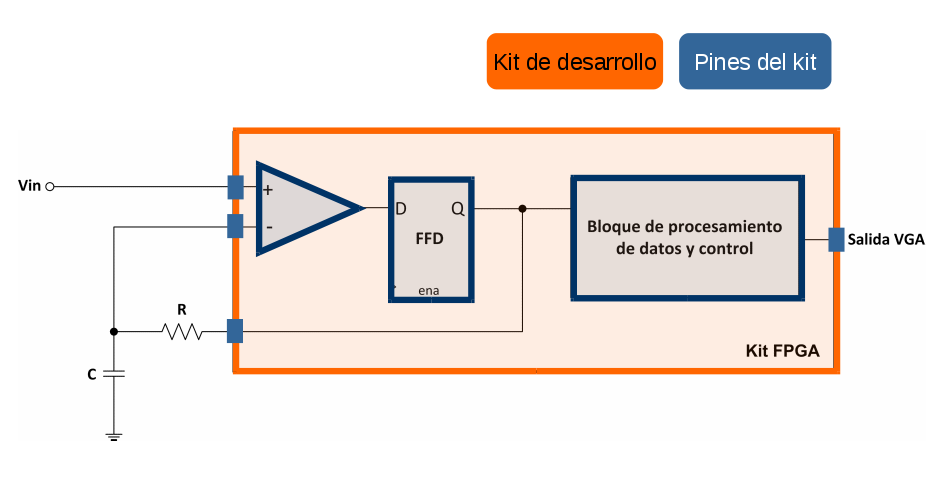
\includegraphics[scale=0.5]{./imagenes/bloques_general.png}
\caption{Diagrama en bloques general}
 \label{fig:bloques_general}
\end{center}
\end{figure}

\subsection{Diagrama en bloques del procesamiento y control}

En la figura \ref{fig:bloques_control} se presenta el diagrama en bloques
del procesamiento y control del voltímetro.
Este bloque es el encargado de obtener en base al PWM recibido la tensión
$V_{in}$ y codificar dicho valor en un contador BCD de 3 digitos, y
mostrar el resultado por salida VGA.

\begin{figure}[H] %[h] para here [b] para bottom [t] para top [H]+float para aqui si o si
\begin{center}
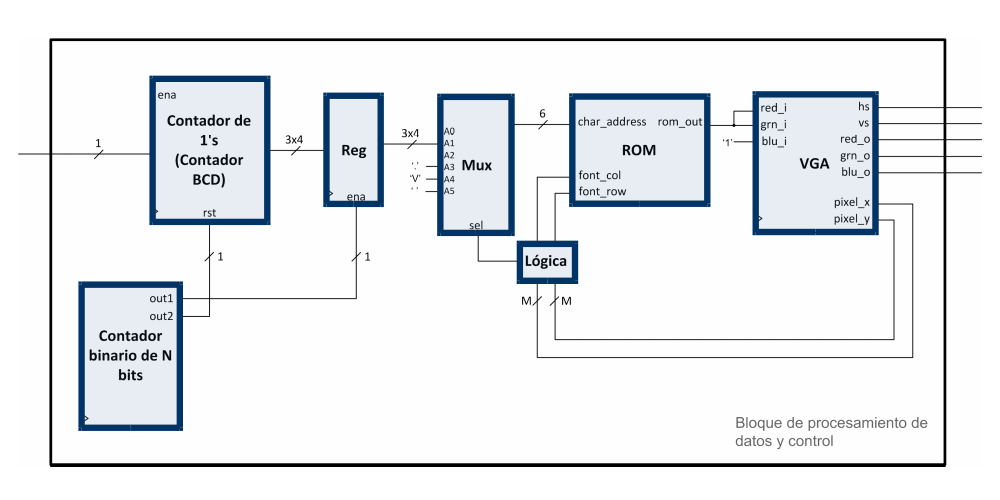
\includegraphics[scale=0.5]{./imagenes/bloques_control.png}
\caption{Diagrama en bloques del procesamiento y control}
 \label{fig:bloques_control}
\end{center}
\end{figure}

\subsection{Contador BCD}

Es un contador BCD de 3 digitos, cuenta los ciclos de reloj en que
la entrada recibida se encuentra en 1.
Cuenta con una entrada \texttt{rst} para ser reiniciado.

\subsection{Contador binario de N bits}

Siendo N = 9 bits, este contador cuenta 330 ciclos de reloj, para luego
guardar la salida del contador BCD en el registro y finalmente reiniciar
el contador BCD.
Notar que si la entrada del contador BCD es un PWM del $100\,\unit{\%}$
la salida del contador BCD será 330 (en decimal) en el momento en el que
el contador binario de N bits haya contado los 330 ciclos de reloj.
Si el PWM es del $50\,\unit{\%}$ el contador BCD solo contará 165 ciclos
para cuando se guarde su valor en el registro.

\subsection{Multiplexor}

El multiplexor es utilizado por el bloque \texttt{Lógica} para seleccionar
el caracter que se necesite mostrar por pantalla.

\subsection{ROM}

En la memoria ROM serán guardadas las estructuras de los carácteres
necesarios para mostrar el resultado por pantalla. Estos son los números
del `0' al '9', ' ', ',' y 'V'.

\subsection{Lógica}

Este bloque recibe la fila y columna del pixel actual del bloque "VGA"
y en base a este dato deberá seleccionar el carácter que deba ser mostrado.
En caso de no estar en un pixel correspondiente a la mediciòn del voltímetro
seleccionará el caracter ' ' utilizando el multiplexor.

\section{Simulaciones}

A continuación se muestran algunas simulaciones realizadas mediante pruebas.

\subsection{Contador BCD}

En esta simulación se comprobó que el contador BCD cuenta como un número
decimal de 3 dígitos, cada dígito esta representado por 4 bits.

\begin{figure}[H] %[h] para here [b] para bottom [t] para top [H]+float para aqui si o si
\begin{center}
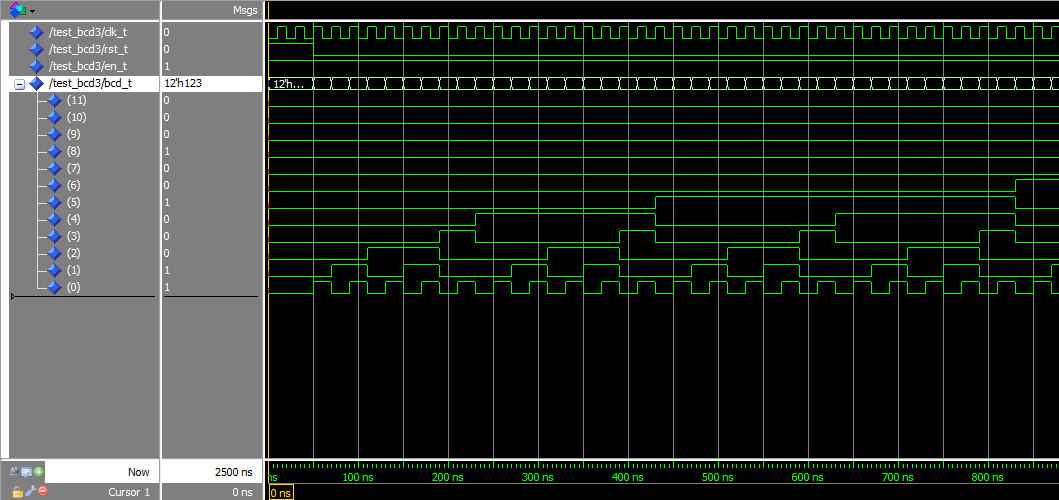
\includegraphics[scale=0.5]{./imagenes/bcd3_test.png}
\caption{Simulación del contador BCD}
 \label{fig:sim_bcd}
\end{center}
\end{figure}


\subsection{Contador binario de N bits}

Se verificó que los flags de salida de este bloque se ejecuten en el
orden necesario. Como se verifica en la figura \ref{fig:sim_counter}
primero se habilita el flag \texttt{out\_1} que corresponde al registro,
guardando así el valor de la salida del contador BCD en ese momento.
Paso siguiente reinicia el contador BCD.

\begin{figure}[H] %[h] para here [b] para bottom [t] para top [H]+float para aqui si o si
\begin{center}
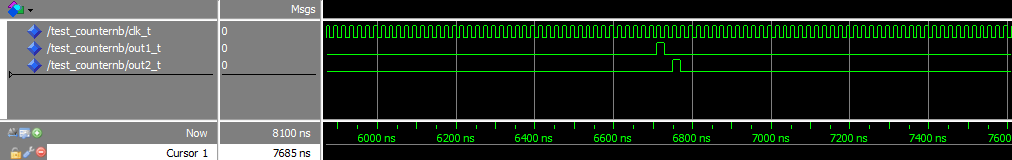
\includegraphics[scale=0.5]{./imagenes/Counter_test.png}
\caption{Simulación del contador binario de N bits}
 \label{fig:sim_counter}
\end{center}
\end{figure}


\subsection{Multiplexor}

Las entradas del multiplexor eran: ``0000'', ``0000'', ``1000'', ``0100'', ``0010''
y ``0001''. se fue incrementando en 1 los bits de selección desde 0 hasta
3. Se verificó que la salida del multiplexor correspondía a la
siguiente secuencia: ``0001'', ``0010'', ``0100'' y ``1000''.

\begin{figure}[H] %[h] para here [b] para bottom [t] para top [H]+float para aqui si o si
\begin{center}
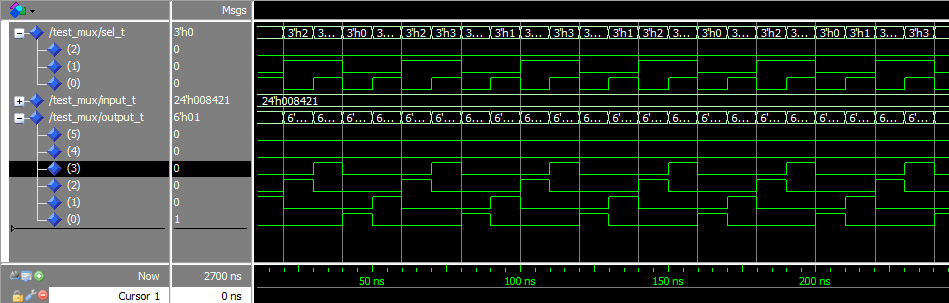
\includegraphics[scale=0.5]{./imagenes/mux_test.png}
\caption{Simulación del multiplexor}
 \label{fig:sim_mux}
\end{center}
\end{figure}


\subsection{Registro}

Se verificó que la salida del registro es igual a la entrada cuando
el flag \texttt{en\_t} valía 1. Cuando valía 0 guardaba el último dato
mostrado.

\begin{figure}[H] %[h] para here [b] para bottom [t] para top [H]+float para aqui si o si
\begin{center}
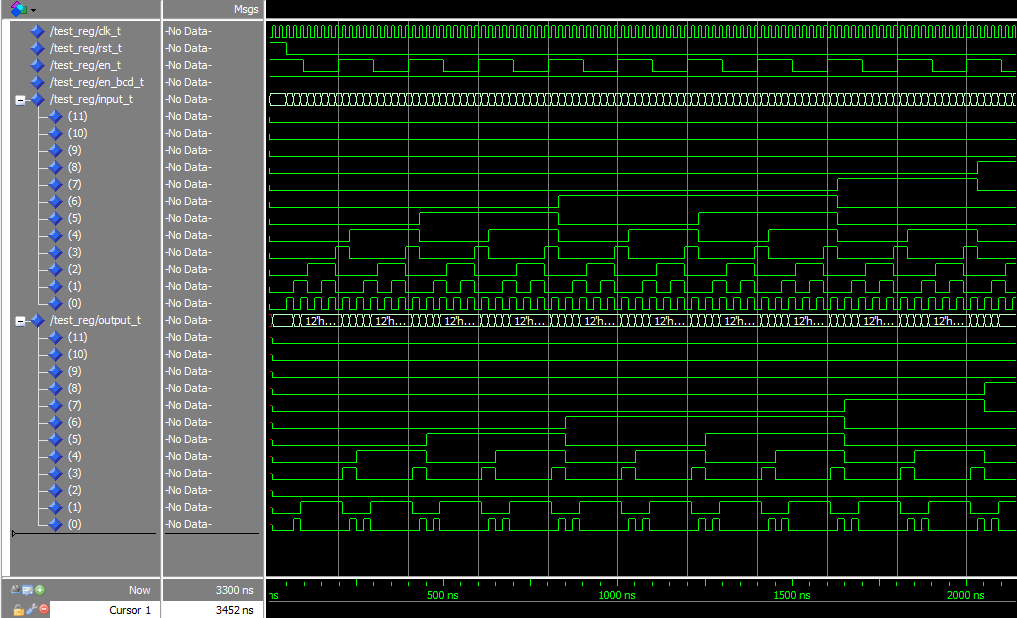
\includegraphics[scale=0.5]{./imagenes/reg_test.png}
\caption{Simulación del registro}
 \label{fig:sim_reg}
\end{center}
\end{figure}


\subsection{Sampler}

Este bloque esta compuesto por el contador BCD, el contador binario
de N bits y el registro.
Se ingresó un PWM de $80\,\unit{\%}$ y se verificó que la salida era
265, valor que corresponde a $2.65\,\unit{V}$. Se puede comprobar que
si un PWM del $100\,\unit{\%}$ corresponde a $3.30\,\unit{V}$ entonces
un PWM del $80\,\unit{\%}$ corresponde a $2.64\,\unit{V}$

\begin{figure}[H] %[h] para here [b] para bottom [t] para top [H]+float para aqui si o si
\begin{center}
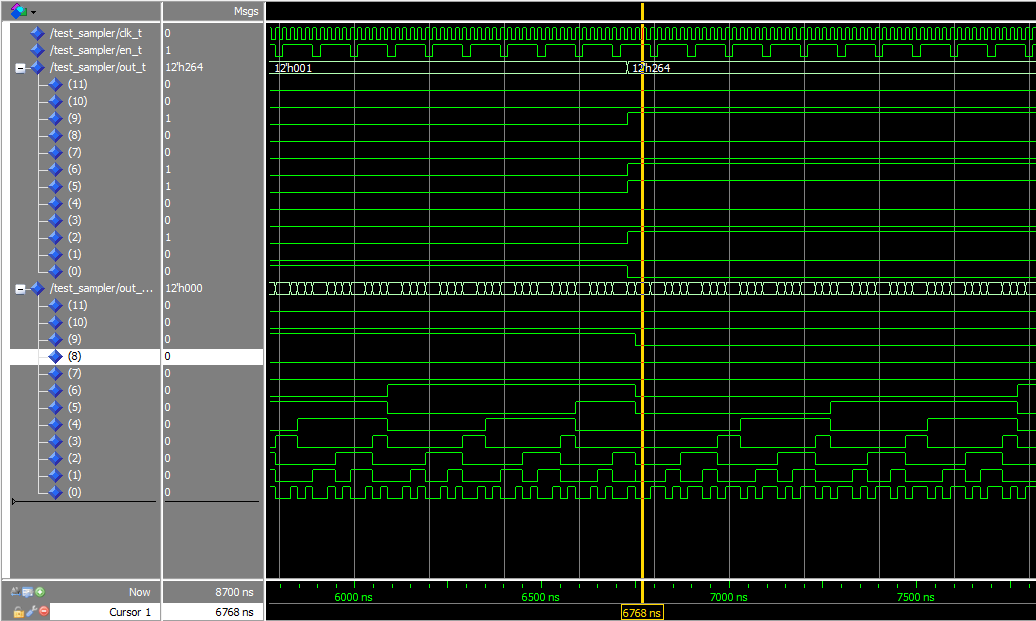
\includegraphics[scale=0.5]{./imagenes/sampler_test.png}
\caption{Simulación del sampler}
 \label{fig:sim_sampler}
\end{center}
\end{figure}


\section{Resumen de síntesis}

\begin{center}
\begin{tabular}{|c|c|c|}\hline
Utilización Lógica & Usados & Utilización \\\hline
Slices & $116$ & $2\, \unit{\%}$ \\\hline
Flip-Flops & $65$ & $0\, \unit{\%}$ \\\hline
LUTs & $213$ & $2\, \unit{\%}$ \\\hline
GCLK  & $1$ & $4\, \unit{\%}$ \\\hline
\end{tabular}
\end{center}

\newpage
\section{Código fuente VHDL}

\subsection{BCD.vhd}
\lstinputlisting[language=VHDL]{../codigo/BCD.vhd}
\newpage

\subsection{BCD3.vhd}
\lstinputlisting[language=VHDL]{../codigo/BCD3.vhd}
\newpage

\subsection{BCD3\_test.vhd}
\lstinputlisting[language=VHDL]{../codigo/BCD3_test.vhd}
\newpage

\subsection{Char\_ROM.vhd}
\lstinputlisting[language=VHDL]{../codigo/Char_ROM.vhd}
\newpage

\subsection{CounterNb.vhd}
\lstinputlisting[language=VHDL]{../codigo/CounterNb.vhd}
\newpage

\subsection{CounterNb\_test.vhd}
\lstinputlisting[language=VHDL]{../codigo/CounterNb_test.vhd}
\newpage

\subsection{FFD.vhd}
\lstinputlisting[language=VHDL]{../codigo/FFD.vhd}
\newpage

\subsection{Logic.vhd}
\lstinputlisting[language=VHDL]{../codigo/Logic.vhd}
\newpage

\subsection{Mux.vhd}
\lstinputlisting[language=VHDL]{../codigo/Mux.vhd}
\newpage

\subsection{Mux\_gen.vhd}
\lstinputlisting[language=VHDL]{../codigo/Mux_gen.vhd}
\newpage

\subsection{Mux\_test.vhd}
\lstinputlisting[language=VHDL]{../codigo/Mux_test.vhd}
\newpage

\subsection{Process\_and\_controll.vhd}
\lstinputlisting[language=VHDL]{../codigo/Process_and_controll.vhd}
\newpage

\subsection{Reg.vhd}
\lstinputlisting[language=VHDL]{../codigo/Reg.vhd}
\newpage

\subsection{Reg\_test.vhd}
\lstinputlisting[language=VHDL]{../codigo/Reg_test.vhd}
\newpage

\subsection{Sampler.vhd}
\lstinputlisting[language=VHDL]{../codigo/Sampler.vhd}
\newpage

\subsection{Sampler\_test.vhd}
\lstinputlisting[language=VHDL]{../codigo/Sampler_test.vhd}
\newpage

\subsection{VGActrl.vhd}
\lstinputlisting[language=VHDL]{../codigo/VGActrl.vhd}
\newpage

\subsection{VGA\_volt.vhd}
\lstinputlisting[language=VHDL]{../codigo/VGA_volt.vhd}
\newpage

\subsection{Volt.vhd}
\lstinputlisting[language=VHDL]{../codigo/Volt.vhd}
\newpage

\end{document}
